

\documentclass[14pt,a4paper]{scrartcl}

\usepackage[ngerman]{babel}
\usepackage[utf8]{inputenc}
\usepackage{lmodern}
\usepackage[T1]{fontenc}
\usepackage[autostyle=true, german=quotes]{csquotes}
\usepackage[square,numbers]{natbib}
\usepackage{hyperref}
\usepackage{graphicx}
\usepackage{bookmark}
\usepackage{amsmath}

\setlength{\parindent}{0pt}
\setlength{\parskip}{1ex}

\begin{document}

\begin{titlepage}
\begin{center}

\vspace*{2cm}


\includegraphics[width=10cm]{figures/fernuni_logo.png}

\vspace{3cm}

Seminararbeit zum Thema:\\[1.5em]
\textbf{Fehlertoleranz und Robustheit eines
komplexen Smart-Grid-Netzwerks
}\\[4em]

Fakultät für Mathematik und Informatik\\
FernUniversität in Hagen\\[5em]

eingereicht bei:\\
apl. Prof. Dr. Zhong Li\\[5em]

eingereicht von:\\
Aymane Bouchaara, 3529908\\
Carina Vetter, 2153378\\
Bianca Schwob, 7659954\\[3em]





Abgabedatum: 04.01.2026

\end{center}
\end{titlepage}

\pagenumbering{Roman}

\tableofcontents
\clearpage

\pagenumbering{arabic}

\section{Einleitung}
Durch die fortschreitende Digitalisierung und den zunehmenden Ausbau dezentraler 
Energiequellen befinden sich Stromnetze heute in einem großen Wandel. 
Sie entwickeln sich zu Smart Grids. Diese zeichnen sich dadurch aus, 
dass sie physische Energieinfrastruktur mit Informations- und 
Kommunikationstechnologie verbinden. Das soll, trotz schwankender Einspeisung aus 
erneuerbaren Energien und dynamischer Lastprofile, einen stabilen und effizienten 
Netzbetrieb gewährleisten \citep[S.529]{Gungor2013SmartGrid}. Smart Grids unterscheiden 
sich von herkömmlichen Stromnetzen. Letztere waren meist hierarchisch organisiert 
und auf zentrale Energieerzeugung sowie unidirektionale Energieflüsse ausgelegt. 
Im Gegensatz dazu bieten Smart Grids hohe Dezentralität, bidirektionale Energieflüsse,
 Informationsflüsse und adaptive Steuerungsmechanismen \citep[S. 12]{Appelrath2012SmartGrid}.

Diese zunehmende Vernetzung und Abhängigkeiten der Komponenten führt jedoch nicht nur
 zu höherer Effizienz, sondern auch zu einer größeren Verwundbarkeit des Systems. 
 Störungen durch zufällige Ausfälle, wie Überlastungen oder auch gezielte Angriffe 
 auf bestimmte Knotenpunkte, können sich aufgrund der wechselseitigen 
 Interdependenzen schnell zu großflächigen Ausfällen ausbreiten und zu 
 Versorgungsstörungen im ganzen Netz entwickeln \citep[S. 1025]{Buldyrev2010Interdependent}. 
 Gerade die enge Zusammenarbeit von physischen und digitalen Netzen macht Smart Grids 
 anfällig für kaskadierende Effekte, die mit Analysen von konventionellen Stromnetzen 
 nicht ausreichend erfasst werden können.
Vor diesem Hintergrund gewinnt der Begriff der Resilienz ganz besonders an Bedeutung,
 denn er beschreibt die Fähigkeit eines Systems Störungen zu absorbieren und seine grundlegende Funktion aufrechtzuerhalten oder sich nach einem Ausfall wieder zu erholen \citep[S. 17]{Holling1973Resilience}. Zur systematischen Analyse dieser Eigenschaften bietet die Theorie komplexer Netzwerke einen geeigneten methodischen Rahmen.
Für die Fehlertoleranz und Robustheit des Systems spielt dabei die Struktur des Netzwerks eine wichtige Rolle. Denn unterschiedliche Topologien, wie zufällige Netzwerke, Smallworld- oder Skalenfreie Netzwerke, weisen unterschiedliche charakteristische Muster auf und gehen unterschiedlich mit zufälligen Ausfällen und gezielten Angriffen um. Insbesondere unterscheiden sich die Rollen hochvernetzter Knoten und die Fragmentierung der Netzwerke \citep[S. 105ff]{Albert2000ErrorAttack}.
Ausgehend davon verfolgt diese Arbeit das Ziel, die folgende Leitfrage zu untersuchen: „Wie beeinflusst die Netzwerkstruktur eines Smart Grids die Fehlertoleranz beziehungsweise die Robustheit gegenüber zufälligen Ausfällen und gezielten Angriffen?“ Mithilfe netzwerkbasierter Methoden werden dazu unterschiedliche Störszenarien simuliert und geeignete Resilienzmetriken berechnet, um strukturelle Einflussfaktoren zu identifizieren und Ansatzpunkte zur gezielten Verbesserung der Netzstabilität aufzuzeigen.

\section{Theoretische Grundlagen}
\subsection{Smart Grids als komplexe Netzwerke}
Wie in der Einleitung bereits geschrieben stellen Smart Grids eine Weiterentwicklung konventioneller Stromnetze dar. Sie können als cyber-physische-Systeme , in denen physische Komponenten wie Kraftwerke, Umspannwerke oder Leitungen eng mit digitalen Kommunikations- und Steuerungseinheiten interagieren verstanden werden. Entscheidungen über Lastverteilung, Einspeisung oder Netzstabilisierung erfolgen zunehmend automatisiert und datengetrieben, wodurch neue Abhängigkeiten zwischen räumlich und funktional getrennten Netzkomponenten entstehen. Störungen können sich daher nicht nur entlang physischer Leitungen ausbreiten, sondern auch über informationstechnische Kanäle verstärkt oder ausgelöst werden.
Zur Analyse dieser komplexen Wechselwirkungen bietet sich eine Abstraktion von Smart Grids als Netzwerke an. In dieser Darstellung werden physische oder logische Komponenten des Stromnetzes als Knoten modelliert, während elektrische Leitungen, Kommunikationsverbindungen oder funktionale Abhängigkeiten als Kanten beschrieben werden. Eine solche graphbasierte Modellierung erlaubt es, strukturelle Eigenschaften des Gesamtsystems systematisch zu erfassen und vergleichbar zu machen. Insbesondere ermöglicht sie die Untersuchung, wie die Anordnung und Vernetzung der Komponenten die Stabilität, Fehlertoleranz und Resilienz des Netzes beeinflussen.
Die Anwendung der Theorie komplexer Netzwerke ist dabei nicht als Vereinfachung realer Stromnetze zu verstehen, sondern als analytischer Rahmen, der gezielt jene Aspekte hervorhebt, die für das Verhalten vernetzter Systeme unter Störungen entscheidend sind. Resilienz in Smart Grids wird maßgeblich durch die Struktur der Verbindungen bestimmt, über die sich Ausfälle, Überlastungen oder Fehlfunktionen ausbreiten oder abgefedert werden können. Netzwerkbasierte Ansätze ermöglichen es somit, strukturelle Ursachen von Verwundbarkeit zu identifizieren, ohne sich ausschließlich auf detaillierte physikalische Simulationsmodelle stützen zu müssen.
Gerade im Kontext zunehmender Dezentralität und Komplexität bieten netzwerktheoretische Methoden einen wichtigen Mehrwert, da sie den Fokus auf systemische Eigenschaften legen. Sie erlauben es, kritische Komponenten zu identifizieren, strukturelle Schwachstellen aufzudecken und allgemeine Aussagen über die Robustheit des Netzwerks gegenüber unterschiedlichen Störungsszenarien zu treffen. Damit bilden sie eine zentrale theoretische Grundlage für die in dieser Arbeit verfolgte Resilienzanalyse von Smart Grids.

\subsection{Netzwerkmodelle und strukturelle Eigenschaften}
Die Struktur eines Netzwerks hat einen entscheidenden Einfluss darauf, wie robust oder verwundbar es gegenüber Störungen ist. Um diese Zusammenhänge systematisch zu untersuchen, wurden in der Netzwerktheorie verschiedene Modellklassen entwickelt, die charakteristische Topologien realer Systeme abstrahieren. Ergänzend dazu ermöglichen strukturelle Netzwerkmetriken eine quantitative Beschreibung dieser Topologien und dienen als Erklärgrößen für das Verhalten von Netzwerken unter Ausfällen oder Angriffen.
\subsubsection{Netzwerktopologien}
Komplexe Netzwerke können auf unterschiedliche Weise strukturiert sein. Drei grundlegende Modelle haben sich bisher zur Beschreibung und Simulation realer Systeme etabliert: Erdős-Rényi-Netzwerke, Watts-Strogatz-Small-World-Netzwerke und Barabási-Albert-skalenfreie Netzwerke. Diese Topologien unterscheiden sich hinsichtlich Verbindungsstruktur, Gradverteilung, Clusterkoeffizient und typischer Pfadlängen und damit auch hinsichtlich ihrer Resilienz.
Das Erdős-Rényi-Netzwerk, ER-Modell, \citep{Erdos1959RandomGraphs} erzeugt ein Netzwerk, indem zwischen allen möglichen Knotenpaaren jeweils mit einer festen Wahrscheinlichkeit p eine Kante gezogen wird. Diese zufällige Verbindungsstrategie hat mehrere Konsequenzen:
	Die Gradverteilung ist binomial- bzw. in großen Netzen näherungsweise Poisson-verteilt und die meisten Knoten haben ähnliche Gradwerte.
	Der Clusterkoeffizient ist vergleichsweise gering, da nur wenige Dreiecksbeziehungen entstehen.
	Die Pfadlänge ist typischerweise klein (logarithmisch mit Netzwerkgröße).
	Die Resilienz ist moderat robust gegenüber zufälligen Ausfällen, aber vulnerabel gegenüber gezielten Angriffen, da keine systematische Struktur existiert, die kritische Knoten schützt.
ER-Netzwerke bilden eine wichtige Baseline, aber reale Stromnetze weisen häufig strukturierte Muster auf, die durch dieses Modell nicht vollständig beschrieben werden können.
Das Small-World-Netzwerk-Modell \citep{Watts1998SmallWorld} kombiniert Merkmale regulärer und zufälliger Netzwerke. Die Konstruktion erfolgt durch Ausgang eines regulären Rings, in dem Knoten mit ihren nächsten Nachbarn verbunden sind, und anschließend eine zufällige „Umverteilung“ einzelner Kanten passiert.
Charakteristische Eigenschaften:
	Eine hohe lokale Clusterbildung - also eine lokale Redundanz - wird geschaffen. Diese Knoten haben viele gemeinsame Nachbarn.
	Die durchschnittliche Pfadlänge ist eher kurz. Dadurch existiert eine effiziente Erreichbarkeit im gesamten Netzwerk.
	Die Resilienz ist durch hohe lokale Clusterung vergleichsweise hoch und damit das Netzwerk widerstandsfähiger gegenüber Ausfällen. Jedoch ist es anfällig für Störungen, wenn die wenigen „Shortcut“-Kanten ausfallen, die die Pfadlänge stark reduzieren.
Small-World-Strukturen treten in vielen Energie- und Informationsnetzen auf, da sie Effizienz mit lokaler Stabilität verbinden.
Von besonderer Bedeutung sind skalenfreie Netzwerke nach Barabási und Albert, deren Knotengradverteilung einem Potenzgesetz folgt. Das BA-Modell \citep{Albert2000ErrorAttack} basiert auf „präferentieller Komplexe Netzwerke können auf unterschiedliche Weise strukturiert sein. Drei grundlegende Modelle haben sich bisher zur Beschreibung und Simulation realer Systeme etabliert: Erdős-Rényi-Netzwerke, Watts-Strogatz-Small-World-Netzwerke und Barabási-Albert-skalenfreie Netzwerke. Diese Topologien unterscheiden sich hinsichtlich Verbindungsstruktur, Gradverteilung, Clusterkoeffizient und typischer Pfadlängen und damit auch hinsichtlich ihrer Resilienz.
Das Erdős-Rényi-Netzwerk, ER-Modell, \citep{Erdos1959RandomGraphs} erzeugt ein Netzwerk, indem zwischen allen möglichen Knotenpaaren jeweils mit einer festen Wahrscheinlichkeit p eine Kante gezogen wird. Diese zufällige Verbindungsstrategie hat mehrere Konsequenzen:
	Die Gradverteilung ist binomial- bzw. in großen Netzen näherungsweise Poisson-verteilt und die meisten Knoten haben ähnliche Gradwerte.
	Der Clusterkoeffizient ist vergleichsweise gering, da nur wenige Dreiecksbeziehungen entstehen.
	Die Pfadlänge ist typischerweise klein (logarithmisch mit Netzwerkgröße).
	Die Resilienz ist moderat robust gegenüber zufälligen Ausfällen, aber vulnerabel gegenüber gezielten Angriffen, da keine systematische Struktur existiert, die kritische Knoten schützt.
ER-Netzwerke bilden eine wichtige Baseline, aber reale Stromnetze weisen häufig strukturierte Muster auf, die durch dieses Modell nicht vollständig beschrieben werden können.
Das Small-World-Netzwerk-Modell \citep{Watts1998SmallWorld} kombiniert Merkmale regulärer und zufälliger Netzwerke. Die Konstruktion erfolgt durch Ausgang eines regulären Rings, in dem Knoten mit ihren nächsten Nachbarn verbunden sind, und anschließend eine zufällige „Umverteilung“ einzelner Kanten passiert.
Charakteristische Eigenschaften:
	Eine hohe lokale Clusterbildung - also eine lokale Redundanz - wird geschaffen. Diese Knoten haben viele gemeinsame Nachbarn.
	Die durchschnittliche Pfadlänge ist eher kurz. Dadurch existiert eine effiziente Erreichbarkeit im gesamten Netzwerk.
	Die Resilienz ist durch hohe lokale Clusterung vergleichsweise hoch und damit das Netzwerk widerstandsfähiger gegenüber Ausfällen. Jedoch ist es anfällig für Störungen, wenn die wenigen „Shortcut“-Kanten ausfallen, die die Pfadlänge stark reduzieren.
Small-World-Strukturen treten in vielen Energie- und Informationsnetzen auf, da sie Effizienz mit lokaler Stabilität verbinden.
Von besonderer Bedeutung sind skalenfreie Netzwerke nach Barabási und Albert, deren Knotengradverteilung einem Potenzgesetz folgt. Das BA-Modell \citep{Albert2000ErrorAttack} basiert auf „präferentieller Anbindung“ von Knoten. Es werden nacheinander Knoten hinzugefügt und sie werden bevorzugt mit bereits gut vernetzten Knoten verbunden („the rich get richer“). Dadurch entstehen sog. Hubs.
Eigenschaften:
	Die Gradverteilung folgt einem Potenzgesetz (scale-free). Dadurch entstehen wenige Hubs mit vielen Knoten mit geringem Grad.
	Der Clusterkoeffizient ist vergleichsweise gering, kann aber je nach Erweiterung variieren.
	Die Pfadlängen ist sehr kurz, da Hubs viele Wege verbinden (ultra-small world).
	Die Resilienz ist hoch, da das Netzwerk sehr robust gegen zufällige Ausfälle ist (da diese meist kleine Knoten betreffen). Es ist aber stark anfällig gegenüber gezielten Angriffen auf Hubs, da das Netzwerk leicht fragmentieren kann.
Viele reale Infrastrukturnetze, einschließlich Kommunikationssysteme, Internet-Backbones und Teile moderner Stromnetze, zeigen skalenfreie Eigenschaften. Daher ist das BA-Modell besonders relevant für Analysen der Verwundbarkeit kritischer Infrastrukturen.

\subsubsection{Strukturelle Netzwerkmetriken}

Um die Robustheit und Verwundbarkeit eines Netzwerks quantitativ zu beschreiben, werden verschiedene strukturelle Metriken herangezogen. Eine zentrale Rolle spielt dabei die Gradverteilung.
Die Gradverteilung $P(k)$ ist die Wahrscheinlichkeit, dass ein Knoten eines Netzwerks Grad k hat und liegt zwischen 0 und 1. Die Gradverteilung eines Netzwerks zeigt die Beschaffenheit deren Gesamtstruktur auf und kann somit der Feststellung damit einhergehender, typischer Eigenschaften dienen. Für Smart Grids ist die Feststellung solcher typischen Eigenschaften insofern relevant, als dass hierdurch kritische Hubs identifiziert werden können, wie z.B. große Umspannwerke mit einer besonders hohen Anzahl an Leitungsverbindungen. Die Gradverteilung von Stromnetzwerken weist die grundsätzlichen Bedingungen der Skalenfreiheit auf: Zum Einen ist durch stetigen Ausbau des Stromnetzes das Wachstum als Voraussetzung gegeben. Ebenso werden die Kraftwerke vorzugsweise über stärker vernetzte Umspannwerke angebunden, anstatt peripher dezentral geleitet zu werden. Somit entsteht die typische Gradverteilung, die dem Potenzgesetz entspricht $P(k) ~ k-\gamma$. Bei dieser Verteilung wird die Wahrscheinlichkeit $P(k)$ bei wachsendem k immer kleiner. Im Falle von Stromnetzwerken, bspw. in der westlichen USA, liegt $\gamma$ ca. bei 4 und somit an der Grenze der Eigenschaften der Skalenfreiheit : die Anzahl großer Hubs ist vergleichsweise gering und stößt mit einer Gesamtzahl von einigen tausend Kraftwerken relativ schnell an eine natürliche Obergrenze. 
Der Clustering-Koeffizient C beschreibt, ob zwei Nachbarn eines Knotens ebenfalls füreinander Nachbarn sind und damit die Ausprägung der Transitivität des Netzwerkes : 
\[
C = \frac{\text{Anzahl geschlossener Pfade der L\"ange 2}}{\text{Anzahl Pfade der L\"ange 2}}
\]
Bei einer sehr großen Anzahl an Knoten N eines Netzwerks wird der Clustering-Koeffizient sehr klein. Diese Ausprägung eines Extremfalls ist bei Stromnetzen aufgrund der begrenzten Knotenanzahl jedoch nicht gegeben. Relevant wird der Clustering-Koeffizient dann, wenn einzelne Knoten und Verbindungen ausfallen. Der Koeffizient gibt an, wie groß die Redundanz im Netzwerk ist. Ist ein hoher Clustering-Koeffizient gegeben, so stehen im Netzwerk mehrere alternative Pfade bei Ausfällen zur Verfügung, was für Robustheit des Netzwerks gegen lokale Ausfälle sorgt. 
Die mittlere Pfadlänge beschreibt die mittlere kürzeste Entfernung zwischen Knoten. Dieser Kennwert ist relevant, um die Ausbreitung von Lastfluss oder Störungen zu beschreiben und um die Wiederherstellungszeit einzuschätzen . Die mittlere Pfadlänge lässt sich wie folgt berechen:
\[
\ell = \frac{1}{N(N-1)} \sum_{i j} d_{i j}
\]
Wobei $d_{ij}$ die durchschnittliche kürzeste Distanz zwischen den Knoten i und j eines Netzwerks bezeichnet.

\subsection{Robustheit, Resilienz, Fehlertoleranz}
In der Literatur zu komplexen Netzwerken werden die Begriffe Robustheit, Fehlertoleranz und Resilienz häufig gemeinsam verwendet, obwohl diese verschiedene Schwerpunkte fokussieren. In den folgenden Unterkapiteln wird eine Abgrenzung im Kontext von Stromnetzwerken vorgenommen, basierend auf der Übersichtsarbeit von Xiaoyu Qi und Gang Mei (2024). 
\subsubsection{Robustheit}
Robustheit beschreibt die Fähigkeit eines Netzwerks, seine Strukturen und Funktionen trotz Störungen weitgehend gleichbleibend aufrechtzuerhalten. Robustheit kann als Teilaspekt von Resilienz betrachtet werden  und bezieht sich hauptsächlich darauf, wie widerstandsfähig ein Netzwerk in seiner Struktur selbst gegenüber Störungen ist. Im Bereich von Stromnetzwerken, die zu den technologischen Netzwerken zählen, wird Robustheit als die Resistenz gegenüber Ausfällen bezeichnet. Die Kernfrage der Robustheit besteht darin, wie gut die Netzwerkfunktion unmittelbar nach einer Störung erhalten bleibt. In diesem Sinne gilt ein Stromnetz als robust, sofern der Ausfall eines einzelnen Umspannwerks keine weiterführenden Stromausfälle verursacht. 
Gemessen wird die Robustheit typischer Weise über die größte zusammenhängende Komponente (GCC). Hierbei werden nach und nach Knoten oder Kanten entweder zufällig oder gezielt aus dem Netzwerk entfernt und nach jedem Schritt die Größe des größten funktionierenden Netzteils gemessen : 
\[
\mathrm{Rob} = \frac{1}{N} \sum_{q=1}^{N} S(q)
\]
Wobei Rob die Gesamtrobustheit eines Netzwerks bezeichnet und S(q) die relative Größe der größten Komponente nach q entfernten Knoten darstellt. 
\subsubsection{Fehlertoleranz}
Die Fehlertoleranz bezeichnet die Fähigkeit eines Systems, trotz Fehler einzelner Komponenten weiterhin funktionsfähig zu bleiben und ohne die Fehler zwingend reparieren zu müssen. Während Stromnetze im Bereich der technologischen Netze angesiedelt sind, bezieht sich die Fehlertoleranz mehr auf Informationsnetzwerke, zu denen Kommunikations- und Internetnetzwerke zählen. Dabei wird stärker auf Hard- und Software Bezug genommen und die Fähigkeit beschrieben, Fehler strukturell oder algorithmisch zu kompensieren, z.B. durch Redundanzen oder Umleitung von Flüssen. Die Kernfrage der Fehlertoleranz ist, wie gut das System während eines auftretenden Fehlers weiterarbeiten kann. So gilt ein Stromnetz als fehlertolerant, wenn bei einem Leitungsausfall automatisch alternative Wege für den Stromfluss gewählt werden. 
\subsubsection{Resilienz}
Die Resilienz umfasst die Widerstandsfähigkeit eines Netzwerks im Störungsfall, die Fähigkeit zur Begrenzung der Auswirkungen und die Fähigkeit zur Wiederaufnahme eines akzeptablen Funktionsniveaus. Dementsprechend ist die Resilienz ein übergreifendes Konzept, welches die Robustheit, Fehlertoleranz, Anpassungs- und Erholungsfähigkeit beinhaltet. Ein Smart Grid ist beispielsweise dann resilient, wenn es nach einem extremen Wetterereignis schnell wieder auf ein normales Versorgungsniveau zurückkehren kann. 
Gemessen werden kann die Resilienz anhand der Fläche unter der Leistungs-Zeit-Kurve: 
\[
\mathrm{Res} = \int_{t_0}^{t_1} Q(t)\,\mathrm{d}t
\]
Wobei Q(t) die Systemleistung relativ zur Norm ist und Res beschreibt, wie schnell und wie gut die Erholung erfolgt. Die Leistung kann die Konnektivität (GCC), Flusseffizienz, Versorgungsgrad oder Kommunikationsfähigkeit sein und kann berechnet werden durch 
\[
Q(t) = \frac{P(t)}{TP(t)}
\] wobei P(t) die gemessene und TP(t) die Zielleistung ist, die ohne Störung zu erwarten wäre. 
Bei mehreren Messdurchgängen wird der Erwartungswert von 
\[
\frac{P(t)}{TP(t)}
\] (also der Mittelwert der Messdurchgänge) berechnet. Die Kernfrage der Resilienz ist, wie viel der ursprünglichen Leistung noch vorhanden ist. 

\section{Methodik und Versuchsdesign}

\subsection{Netzwerkmodelle}

Die Untersuchung der Robustheit und Fehlertoleranz von Netzwerken erfordert
eine bewusste Auswahl geeigneter Netzwerkmodelle. Hierbei ist das Ziel, sowohl
abstrakte, kontrollierbare Strukturen als auch realitätsnahe Netze zu
betrachten, um Unterschiede zwischen idealisierten Modellen und realen
Infrastrukturen kenntlich machen zu können. In dieser Arbeit werden daher drei
synthetische Netzwerkmodelle sowie ein reales Stromnetzmodell herangezogen.

\paragraph{Synthetische Netzwerkmodelle:}
Synthetische Netzwerke ermöglichen es, spezifische strukturelle Eigenschaften
gezielt zu variieren und isoliert zu analysieren. Sie dienen als Referenz, um
grundlegende Zusammenhänge zwischen Netzwerkstruktur und Robustheit
systematisch zu untersuchen. 
Als Basismodell wird der Erdős--Rényi-Zufallsgraph verwendet. In diesem Modell
werden $n$ Knoten betrachtet, zwischen denen jede mögliche Kante mit einer
festen Wahrscheinlichkeit $p$ unabhängig von allen anderen Kanten existiert.
Die entstehende Gradverteilung folgt näherungsweise
einer Poisson-Verteilung. Erdős--Rényi-Netzwerke besitzen keine ausgeprägten
Hubs und nur eine geringe lokale Clusterbildung. Dadurch eignen sie sich als
Vergleichsmaßstab für Netzwerke ohne strukturelle Heterogenität.
Das Watts--Strogatz-Modell beschreibt Netzwerke mit Small-World-Eigenschaften, 
also Netzwerke, in denen die meisten Knoten über wenige Schritte erreichbar sind 
(kurze Pfade) und gleichzeitig lokale Cluster mit vielen Verbindungen untereinander existieren.
Ausgangspunkt ist ein reguläres Ringgitter, in dem
jeder Knoten mit $k$ nächsten Nachbarn verbunden ist. Durch zufälliges
Umverdrahten von Kanten mit einer Wahrscheinlichkeit $p$ entstehen kurze
mittlere Pfadlängen bei gleichzeitig erhöhtem Clustering. Diese Eigenschaften
sind insbesondere für technische Infrastrukturnetze relevant, da sie Effizienz
und strukturelle Redundanz kombinieren.\\
Das Barabási--Albert-Modell erzeugt skalenfreie Netzwerke mit einer
potenzgesetzartigen Gradverteilung. Das Modell
basiert auf wachsendem Netzwerkaufbau und bevorzugter Anbindung neuer Knoten an
bereits stark vernetzte Knoten. Dadurch entstehen wenige hochgradige Knoten,
sogenannte Hubs. Skalenfreie Netzwerke gelten als robust gegenüber zufälligen
Ausfällen, zeigen jedoch eine ausgeprägte Anfälligkeit gegenüber gezielten
Angriffen auf zentrale Knoten. Aufgrund dieser
Eigenschaften ist dieses Modell besonders geeignet, um Worst-Case-Szenarien für
Angriffe auf kritische Infrastrukturen zu untersuchen.

\begin{figure}[H]
  \centering
  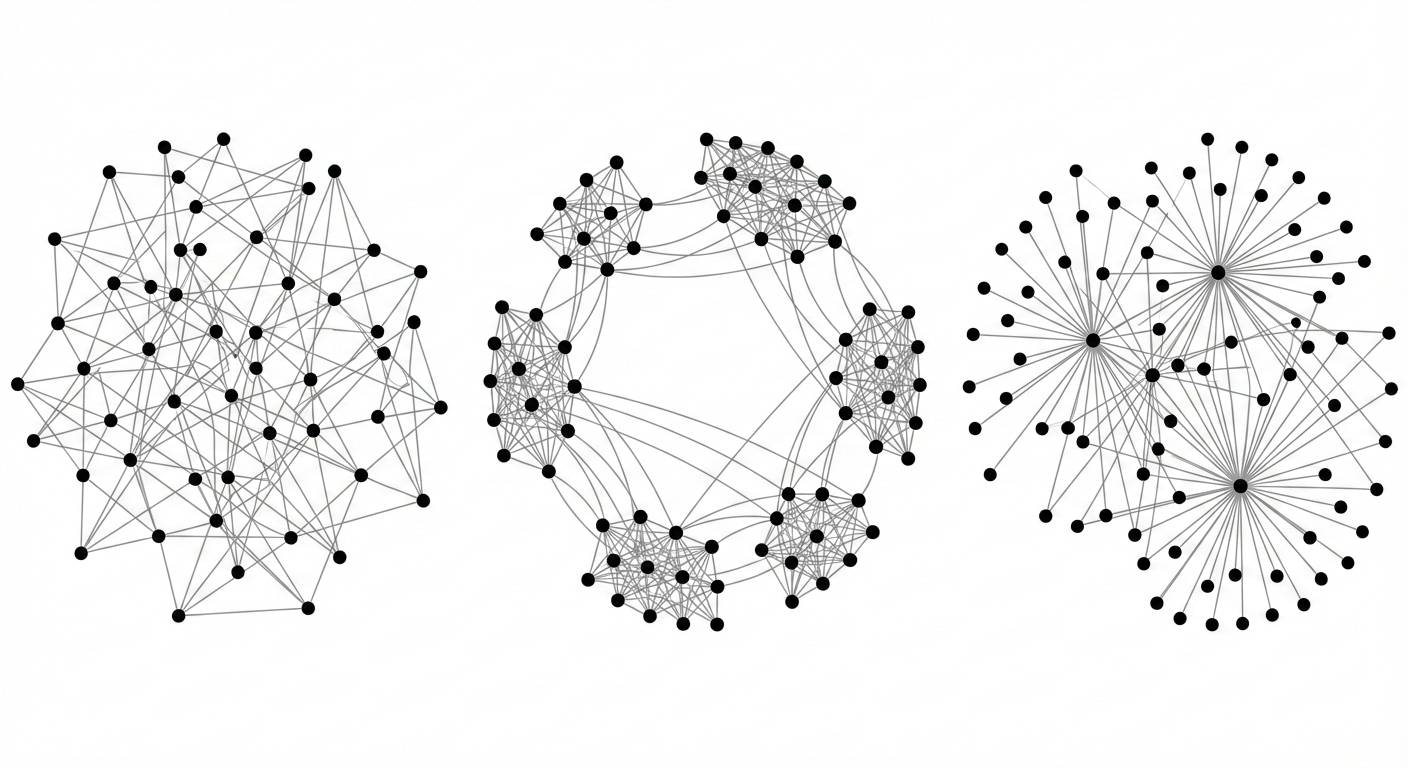
\includegraphics[width=\textwidth]{figures/abb1_NetModelle.png}
  \caption{Vergleich topologischer Netzwerkmodelle. Von links nach rechts:
   Erdős--Rényi-Zufallsgraph (homogene Struktur), 
   Watts--Strogatz-Small-World-Netzwerk (hohe lokale Clusterbildung) 
   und Barabási--Albert-skalenfreies Netzwerk (markante Hub-Struktur).}
  \label{fig:netzwerkmodelle_vergleich}
\end{figure}

\paragraph{Reales Netzwerkmodell:}
Zur Ergänzung der synthetischen Modelle wird ein reales Stromnetz betrachtet.
Als Datengrundlage dient das PyPSA-Eur-Projekt, das ein detailliertes Modell
des europäischen Übertragungsnetzes bereitstellt. 
Die Netzdaten basieren auf öffentlich verfügbaren OpenStreetMap-Informationen und
bilden Hochspannungsleitungen sowie Umspannwerke ab.\\
Für diese Arbeit werden die Netzkomponenten aus den Dateien
\texttt{buses.csv} und \texttt{lines.csv} extrahiert. Um eine einheitliche
Verarbeitung zu ermöglichen, werden die Daten in einen ungerichteten Graphen
überführt und anschließend im GraphML-Format gespeichert. Dieses Format erlaubt
eine direkte Weiterverarbeitung mit gängigen Graphbibliotheken.\\
Die aufbereiteten realen Netzwerke werden im Verzeichnis \texttt{data/real/}
abgelegt, während die ursprünglichen PyPSA-Daten unter \texttt{data/pypsa/}
gespeichert bleiben. Das Laden und optionale Vorverarbeiten der realen Netze,
etwa die Beschränkung auf die größte verbundene Komponente oder die
Umnummerierung der Knoten, erfolgt zentral über die Projektmodule
\texttt{src/graph\_factory.py} und \texttt{src/real\_network\_loader.py}.

\paragraph{Begründung der Modellwahl}
Die Kombination aus synthetischen und realen Netzwerkmodellen ermöglicht einen
strukturierten Vergleich zwischen theoretischen Idealmodellen und realen
Infrastrukturen. Während synthetische Netze gezielte Aussagen über den Einfluss
einzelner Strukturmerkmale erlauben, liefert das reale Stromnetz eine
praxisnahe Referenz. Unterschiede im Robustheits- und
Fehlertoleranzverhalten können so nicht nur quantitativ gemessen, sondern auch
strukturell interpretiert werden. Diese Kombination bildet die Grundlage für
die in den folgenden Abschnitten beschriebenen Störungsszenarien und
Bewertungsmethoden.

\subsection{Störungsszenarien}

Zur Bewertung der Robustheit und Fehlertoleranz komplexer Netzwerke ist nicht
nur die zugrunde liegende Topologie entscheidend, sondern auch die Art der
betrachteten Störungen. Unterschiedliche Ausfallmechanismen können sehr
unterschiedliche Auswirkungen auf die Netzwerkstruktur haben. In dieser Arbeit
werden zwei grundlegende Klassen von Störungsszenarien untersucht: zufällige
Ausfälle einzelner Knoten sowie gezielte Angriffe auf strukturell zentrale
Knoten.

\paragraph{Zufällige Ausfälle (Random Failures)}
Zufällige Ausfälle modellieren Störungen, bei denen einzelne Netzkomponenten
ohne systematische Auswahl ausfallen. Typische Ursachen sind technische
Defekte, altersbedingte Ausfälle oder lokal begrenzte externe Einwirkungen. In
der Simulation werden diese Szenarien durch eine zufällige Auswahl von Knoten
realisiert, die schrittweise aus dem Netzwerk entfernt werden.\\
Formal wird der Ausfallgrad durch den Parameter $q \in [0,1]$ beschrieben, der
den Anteil der entfernten Knoten angibt. Für jeden Wert von $q$ wird eine
entsprechende Anzahl von Knoten zufällig ausgewählt und aus dem ursprünglichen
Netzwerk entfernt. Anschließend werden die strukturellen Eigenschaften des
verbleibenden Netzwerks analysiert.\\
Zufällige Ausfälle dienen in der Netzwerktheorie als Referenzszenario zur
Bewertung der allgemeinen Fehlertoleranz. Insbesondere skalenfreie Netzwerke
zeigen in diesem Fall häufig eine hohe Robustheit, da die Wahrscheinlichkeit
gering ist, dass hochgradige Knoten frühzeitig betroffen sind. Die Ergebnisse aus diesen Szenarien bilden daher eine
wichtige Vergleichsbasis für gezielte Angriffsszenarien.

\paragraph{Gezielte Angriffe auf zentrale Knoten}
Gezielte Angriffe modellieren Störungen, bei denen bewusst solche
Netzkomponenten entfernt werden, die für die Konnektivität oder den Fluss im
Netzwerk von besonderer Bedeutung sind. Diese Szenarien sind insbesondere für
kritische Infrastrukturen relevant, da der Ausfall weniger zentraler Knoten
erhebliche strukturelle Schäden verursachen kann.\\
In dieser Arbeit werden zwei Formen gezielter Angriffe betrachtet. Beim
gradbasierten Angriff werden Knoten in absteigender Reihenfolge ihres
Knotengrads entfernt. Der Knotengrad beschreibt die Anzahl direkter Nachbarn
eines Knotens und dient als einfaches Maß für lokale Vernetzung. Knoten mit
hohem Grad fungieren häufig als Hubs, deren Entfernung zu einer schnellen
Fragmentierung des Netzwerks führen kann.\\
Als zweite Angriffsklasse werden Angriffe auf Basis der Betweenness-Zentralität
untersucht. Die Betweenness-Zentralität misst, wie häufig ein
Knoten auf kürzesten Pfaden zwischen anderen Knoten liegt, und erfasst damit
seine Bedeutung für den globalen Informations- oder Leistungsfluss. Knoten mit
hoher Betweenness wirken häufig als Brücken zwischen ansonsten schwach
verbundenen Teilstrukturen. Ihr Ausfall kann daher selbst bei moderatem
Knotengrad zu einer Aufspaltung des Netzwerks führen.

\paragraph{Implementierung der Störungsszenarien}
Die Umsetzung der Störungsszenarien erfolgt modular innerhalb des Projekts.
Die Bestimmung der Reihenfolge, in der Knoten entfernt werden, ist im Modul
\texttt{src/attacks.py} realisiert. Für zufällige Ausfälle wird eine zufällige
Permutation der Knotenliste erzeugt, während für gezielte Angriffe eine
Sortierung nach dem jeweiligen Zentralitätsmaß erfolgt.\\
Die eigentliche Simulation der Knotenentfernung wird im Modul
\texttt{src/simulation.py} durchgeführt. Für jeden betrachteten Wert von $q$
wird die entsprechende Anzahl von Knoten aus dem Netzwerk entfernt, bevor die
definierten Metriken für das verbleibende Netzwerk berechnet werden. Die klare
Trennung zwischen Angriffsauswahl und Simulation erleichtert die
Nachvollziehbarkeit des Versuchsaufbaus und ermöglicht eine einfache
Erweiterung um zusätzliche Angriffsszenarien.

\paragraph{Begründung der Szenarienauswahl}
Die Kombination aus zufälligen Ausfällen und gezielten Angriffen deckt ein
breites Spektrum realistischer Störungsmechanismen ab. Zufällige Ausfälle
erlauben Aussagen über die allgemeine Fehlertoleranz eines Netzwerks, während
gezielte Angriffe Worst-Case-Szenarien abbilden. Der direkte Vergleich beider
Szenarientypen macht strukturelle Schwächen sichtbar und erlaubt es,
Unterschiede zwischen synthetischen Netzwerkmodellen und realen Stromnetzen
systematisch herauszuarbeiten.


\subsection{Bewertungsmetriken}

Zur quantitativen Bewertung der Robustheit und Fehlertoleranz der
untersuchten Netzwerke werden mehrere komplementäre Metriken herangezogen.
Ziel ist es, sowohl den strukturellen Zerfall des Netzwerks als auch dessen
verbleibende Leistungsfähigkeit unter Störungen abzubilden. Die Auswahl der
Metriken orientiert sich an etablierten Ansätzen der Netzwerktheorie und an
deren praktischer Anwendbarkeit im Kontext von Infrastrukturnetzen.

\paragraph{Größte verbundene Komponente (GCC)}
Eine zentrale Kenngröße zur Bewertung der strukturellen Integrität eines
Netzwerks ist die Größe der größten verbundenen Komponente (Greatest Connected
Component, GCC). Sie beschreibt die Anzahl der Knoten, die nach einer Störung
weiterhin miteinander verbunden sind. Zur Vergleichbarkeit zwischen Netzwerken
unterschiedlicher Größe wird die GCC häufig relativ zur ursprünglichen
Knotenzahl betrachtet.

Formal wird die normierte Größe der größten verbundenen Komponente als


\[
S(q) = \frac{|\text{GCC}(q)|}{N}
\]


definiert, wobei $N$ die ursprüngliche Anzahl der Knoten und $q$ der Anteil der
entfernten Knoten ist. Sinkt $S(q)$ stark ab, deutet dies auf eine
Fragmentierung des Netzwerks hin. Diese Metrik ist besonders geeignet, um
strukturelle Zusammenbrüche zu identifizieren und wird in zahlreichen Arbeiten
zur Robustheitsanalyse verwendet.


\paragraph{Robustheitskurven}
Die Robustheitskurve beschreibt den Verlauf der normierten Größe der größten
verbundenen Komponente $S(q)$ in Abhängigkeit vom Anteil der entfernten Knoten
$q$. Sie stellt somit den schrittweisen Strukturverlust eines Netzwerks unter
zunehmender Störung dar.\\
Robustheitskurven erlauben einen direkten Vergleich unterschiedlicher
Netzwerke und Angriffsszenarien. Flach verlaufende Kurven deuten auf eine hohe
Robustheit hin, während ein steiler Abfall auf eine starke Verwundbarkeit
schließen lässt. Beide Fälle sind schematisch in Abbildung 
\ref{fig:netzwerkmodelle_vergleich} dargestellt. 
In der vorliegenden Arbeit werden Robustheitskurven für
zufällige Ausfälle sowie für gezielte Angriffe berechnet und
gegenübergestellt.\\
Die Berechnung und Visualisierung der Robustheitskurven erfolgt projektintern
im Modul \texttt{src/analysis.py}, wobei die benötigten Rohdaten aus den
Simulationsergebnissen aggregiert werden.

\paragraph{Fläche unter der Robustheitskurve (AUC)}
Zur Verdichtung der Robustheitskurven auf eine einzelne skalare Kennzahl wird
die Fläche unter der Robustheitskurve (Area Under the Curve, AUC) berechnet.
Sie entspricht dem Integral von $S(q)$ über den betrachteten Bereich von $q$
und kann als globales Robustheitsmaß interpretiert werden.\\
Ein hoher AUC-Wert weist darauf hin, dass ein großer Teil des Netzwerks auch
bei fortschreitender Knotenentfernung erhalten bleibt. Umgekehrt signalisiert
ein niedriger AUC-Wert eine hohe Anfälligkeit gegenüber Störungen. Die AUC
erlaubt somit eine kompakte quantitative Bewertung der Robustheit und eignet
sich insbesondere für den Vergleich unterschiedlicher Netzwerke oder
Angriffsszenarien.

\begin{figure}[htbp]
  \centering
  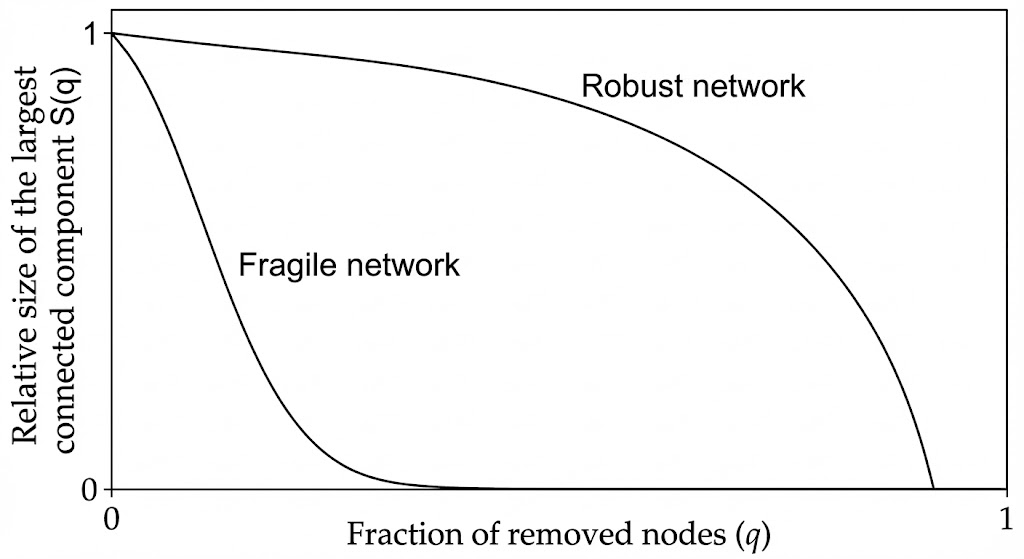
\includegraphics[width=\textwidth]{figures/fragileVsRobustCurves.jpg}
  \caption{Schematische Darstellung von Robustheitskurven für ein robustes
  und ein fragiles Netzwerk.}
  \label{fig:netzwerkmodelle_vergleich}
\end{figure}

\paragraph{Strukturelle Ergänzungsmetriken}
Neben der Größe der größten verbundenen Komponente werden weitere
strukturelle Metriken betrachtet, um das Robustheitsverhalten genauer
einzuordnen. Dazu zählen insbesondere der Clustering-Koeffizient und der
Durchmesser des Netzwerks.\\
Der Clustering-Koeffizient misst den Grad lokaler Vernetzung und dient als
Indikator für strukturelle Redundanz. Ein hoher Clustering-Wert kann auf
alternative Pfade hinweisen, die zur Fehlertoleranz beitragen. In dieser Arbeit
werden sowohl der globale Clustering-Koeffizient als auch der mittlere lokale
Clustering-Koeffizient berechnet.\\
Der Durchmesser beschreibt die maximale kürzeste Pfadlänge zwischen zwei
Knoten innerhalb der größten verbundenen Komponente. Ein stark ansteigender
Durchmesser im Verlauf der Simulation deutet darauf hin, dass das Netzwerk zwar
noch verbunden ist, jedoch an Effizienz verliert. Der Durchmesser ergänzt damit
die GCC-basierte Analyse um eine Aussage zur erreichbaren Netzwerkleistung.

\paragraph{Implementierung der Metriken}
Die Berechnung der beschriebenen Metriken erfolgt zentral im Modul
\texttt{src/metrics.py}. Dieses Modul kapselt alle Metrikfunktionen und stellt
sicher, dass sie konsistent für synthetische und reale Netzwerke angewendet
werden. Die Aggregation der Ergebnisse sowie die Berechnung der AUC erfolgen in
\texttt{src/analysis.py}. Durch diese Trennung zwischen Simulation und
Auswertung wird eine klare Struktur geschaffen, die sowohl die
Nachvollziehbarkeit als auch die Erweiterbarkeit des Projekts unterstützt.

\subsection{Versuchsprotokoll}

Um die Robustheit unterschiedlicher Netzwerke vergleichbar zu untersuchen,
wird ein einheitliches und reproduzierbares Versuchsprotokoll verwendet.
Dieses legt fest, wie Störungen simuliert werden, in welchen Schritten Knoten
entfernt werden und wie die Ergebnisse aggregiert und gespeichert werden. Ziel
ist es, zufällige Effekte zu kontrollieren und belastbare Aussagen über
strukturelle Unterschiede zwischen den Netzwerken zu ermöglichen.

\paragraph{Anzahl der Wiederholungen}
Da insbesondere zufällige Ausfälle und zufällige Netzgenerierung
stochastischen Schwankungen unterliegen, werden Simulationen mehrfach
wiederholt. Für jedes Netzwerkmodell und jedes Störungsszenario werden mehrere
unabhängige Instanzen erzeugt und ausgewertet. Die Anzahl der Wiederholungen
ist dabei konfigurierbar und wird in den jeweiligen Szenariodateien festgelegt.
Die Wiederholungen dienen dazu, zufällige Ausreißer zu glätten und Mittelwerte
über mehrere Läufe zu bilden. Dies ist insbesondere bei Erdős--Rényi- und
Barabási--Albert-Netzwerken relevant, da bereits kleine strukturelle
Unterschiede zwischen einzelnen Instanzen das Robustheitsverhalten
beeinflussen können. Die Aggregation über mehrere Läufe erhöht somit die
statistische Aussagekraft der Ergebnisse.

\paragraph{Schrittweite der Knotenentfernung}
Die Entfernung von Knoten erfolgt schrittweise in Abhängigkeit vom
Ausfallparameter $q$, der den Anteil der entfernten Knoten beschreibt. Die
Schrittweite von $q$ bestimmt die Auflösung der Robustheitskurven. Kleine
Schrittweiten ermöglichen eine feinere Analyse des Netzwerkzerfalls, erhöhen
jedoch den Rechenaufwand.\\
In der vorliegenden Arbeit werden typische Schrittweiten zwischen $0{,}02$ und
$0{,}05$ verwendet. Diese stellen einen Kompromiss zwischen Rechenzeit und
analytischer Genauigkeit dar. Die konkreten Werte werden in den jeweiligen
Konfigurationsdateien definiert und können für einzelne Experimente angepasst
werden.

\paragraph{Aggregation der Ergebnisse}
Die Simulationsergebnisse werden für jeden betrachteten Wert von $q$, jedes
Angriffsszenario und jede Netzwerkinstanz separat erfasst. Zur Auswertung
werden diese Rohdaten anschließend aggregiert. Dabei werden für jede
Kombination aus Netzwerktyp und Angriffsszenario Mittelwerte über alle
Wiederholungen gebildet.\\
Die Aggregation erfolgt insbesondere für die Größe der größten verbundenen
Komponente, aus der die Robustheitskurven $S(q)$ abgeleitet werden. Auf Basis
dieser aggregierten Kurven wird anschließend die Fläche unter der Kurve (AUC)
berechnet. Dieses Vorgehen stellt sicher, dass die Robustheitsbewertung nicht
von einzelnen zufälligen Realisierungen dominiert wird.

\paragraph{Reproduzierbarkeit und Zufallsstartwerte}
Ein zentrales Ziel des Versuchsprotokolls ist die vollständige
Reproduzierbarkeit aller Simulationen. Zu diesem Zweck werden alle
zufallsbasierten Prozesse durch explizite Zufallsstartwerte (Seeds) gesteuert.
Dazu zählen sowohl die Generierung synthetischer Netzwerke als auch die
Auswahl zufälliger Ausfallreihenfolgen bei Random-Failure-Szenarien.\\
Die verwendeten Seeds werden in den jeweiligen Konfigurationsdateien
festgelegt. Dadurch kann jede Simulation exakt reproduziert werden, sofern
dieselben Konfigurationsdateien und dieselbe Softwareversion verwendet werden.
Dieses Vorgehen ist insbesondere für den Vergleich von Ergebnissen und für
eine spätere Nachvollziehbarkeit der Experimente von Bedeutung.

\paragraph{Konfigurations- und Ergebnisstruktur}
Alle experimentellen Parameter werden über YAML-basierte
Konfigurationsdateien im Verzeichnis \texttt{configs/} definiert. Diese
enthalten unter anderem Angaben zu Netzwerkmodellen, Angriffsszenarien,
Schrittweiten, Metriken und Wiederholungszahlen. Durch diese Trennung von
Konfiguration und Code können neue Experimente ohne Anpassung der
Implementierung durchgeführt werden.\\
Die Ergebnisse der Simulationen werden strukturiert im Verzeichnis
\texttt{results/} abgelegt. Für jedes Experiment wird ein eigener Unterordner
erzeugt, der sowohl die Rohdaten der Simulationen als auch aggregierte
Auswertungen enthält. Dieses Vorgehen erleichtert die systematische Analyse
der Ergebnisse und bildet die Grundlage für die in Kapitel~5 dargestellten
Resultate.

\newpage

\section{Implementierung}

\subsection{Werkzeuge und Bibliotheken}

Die Implementierung des praktischen Teils basiert auf einer modularen
Softwarearchitektur in Python. Ziel war es, ein flexibles, reproduzierbares
und erweiterbares Analysewerkzeug zu entwickeln, das sowohl synthetische als
auch reale Netzwerke verarbeiten kann. Die Auswahl der verwendeten Werkzeuge
und Bibliotheken orientiert sich an ihrer Verbreitung in der wissenschaftlichen
Praxis sowie an ihrer Eignung für die Analyse komplexer Netzwerke.

\paragraph{Programmiersprache Python}
Als Programmiersprache wird Python eingesetzt. Python bietet eine gute Balance
zwischen Ausdrucksstärke, Lesbarkeit und Verfügbarkeit wissenschaftlicher
Bibliotheken. Insbesondere für explorative Analysen, Simulationen und
datengetriebene Auswertungen ist Python im Bereich der Netzwerkanalyse weit
verbreitet. Die Implementierung legt Wert auf klare Modulgrenzen und eine
nachvollziehbare Struktur, sodass der Code auch für Dritte leicht verständlich
bleibt.

\paragraph{NetworkX}
Die zentrale Bibliothek für die Modellierung und Analyse der Netzwerke ist
NetworkX. Sie stellt grundlegende Datenstrukturen für Graphen bereit und bietet
eine Vielzahl effizient implementierter Algorithmen zur Berechnung von
Netzwerkmetriken. Dazu zählen unter anderem kürzeste Pfade, Zentralitätsmaße,
Clustering-Koeffizienten sowie Funktionen zur Bestimmung verbundener
Komponenten.\\
Im Projekt wird NetworkX sowohl für die Erzeugung synthetischer Netzwerke als
auch für die Verarbeitung realer Netze verwendet. Durch die einheitliche
Graphrepräsentation können alle Analyse- und Simulationsschritte unabhängig vom
Ursprung des Netzwerks durchgeführt werden.

\paragraph{Datenformate und Dateiverarbeitung}
Zur Speicherung realer Netzwerke wird das GraphML-Format verwendet. GraphML ist
ein XML-basiertes Austauschformat für Graphstrukturen und wird direkt von
NetworkX unterstützt. Dadurch entfällt die Notwendigkeit eigener Parser oder
Konvertierungsroutinen innerhalb der Simulation. Reale Netzwerke, wie das aus
PyPSA-Eur abgeleitete Stromnetz, können so direkt in die Analysepipeline
integriert werden.\\
Konfigurationsdateien werden im YAML-Format abgelegt. YAML ermöglicht eine
übersichtliche und hierarchische Beschreibung experimenteller Parameter und ist
auch für größere Konfigurationen gut lesbar. Die vollständige Parametrisierung
der Experimente erfolgt über diese Dateien, wodurch Änderungen an den
Versuchsbedingungen ohne Anpassung des Programmcodes möglich sind.

\paragraph{Streamlit für die grafische Benutzeroberfläche}
Zur interaktiven Exploration der Simulationsergebnisse wird Streamlit
eingesetzt. Streamlit erlaubt es, mit vergleichsweise geringem
Implementierungsaufwand eine grafische Benutzeroberfläche zu erstellen, die
direkt mit dem Python-Code verbunden ist. Die Benutzeroberfläche dient
insbesondere dazu, Parameter zu variieren, Simulationen zu starten und
Ergebnisse visuell auszuwerten.\\
Ein besonderer Fokus liegt auf der dynamischen Visualisierung der
Netzwerkstruktur während des Simulationsverlaufs. Hierbei werden Knoten und
Kanten des Netzwerks grafisch dargestellt, sodass der schrittweise Zerfall der
Netzwerkstruktur unmittelbar sichtbar wird. Diese visuelle Komponente ergänzt
die numerischen Auswertungen und erleichtert das intuitive Verständnis der
Robustheitsphänomene.

\paragraph{Weitere Hilfsbibliotheken}
Zur numerischen Verarbeitung und Auswertung der Simulationsergebnisse werden
zusätzliche Standardbibliotheken eingesetzt. NumPy dient zur effizienten
Verarbeitung numerischer Daten, während Pandas für das Speichern, Aggregieren
und Weiterverarbeiten der Simulationsergebnisse in Tabellenform verwendet wird.
Matplotlib wird zur Erstellung statischer Plots genutzt, etwa für
Robustheitskurven oder Gradverteilungen außerhalb der interaktiven Oberfläche.

\paragraph{Begründung der Werkzeugwahl}
Die Kombination der genannten Werkzeuge ermöglicht eine klare Trennung zwischen
Modellierung, Simulation, Auswertung und Visualisierung. Gleichzeitig bleibt
das Projekt leichtgewichtig und vollständig auf Open-Source-Komponenten
aufgebaut. Dies unterstützt sowohl die Reproduzierbarkeit der Ergebnisse als
auch die Nachvollziehbarkeit der Implementierung, was insbesondere im
akademischen Kontext von zentraler Bedeutung ist.


\subsection{Softwarearchitektur und Modulaufbau}

Die Software ist modular aufgebaut und folgt einer klaren Trennung zwischen
Konfiguration, Netzwerkgenerierung, Simulation, Auswertung und Visualisierung.
Ziel dieser Struktur ist es, die einzelnen Arbeitsschritte der Analyse
nachvollziehbar zu isolieren und gleichzeitig eine flexible Erweiterbarkeit zu
ermöglichen, gemäß dem Softwaredesignprinzip Seperation of Concerns (SoC). Die Architektur orientiert sich dabei nicht an klassischen
Software-Frameworks, sondern an der logischen Abfolge eines experimentellen
Workflows.

\paragraph{Gesamtstruktur des Projekts}
Das Projekt ist in mehrere Hauptverzeichnisse gegliedert. Der Quellcode
befindet sich im Verzeichnis \texttt{src/}, während Konfigurationsdateien unter
\texttt{configs/} abgelegt sind. Eingabedaten für reale Netzwerke werden in
\texttt{data/} gespeichert, wobei eine Trennung zwischen Rohdaten und
aufbereiteten Graphdateien vorgenommen wird. Simulationsergebnisse werden
strukturiert im Verzeichnis \texttt{results/} abgelegt.
Diese Trennung ermöglicht es, Konfigurationen, Daten und Code unabhängig
voneinander zu verändern. Insbesondere können neue Experimente durch das
Hinzufügen oder Anpassen von YAML-Dateien definiert werden, ohne dass
Änderungen an der Implementierung erforderlich sind.

\begin{figure}[htbp]
  \centering
  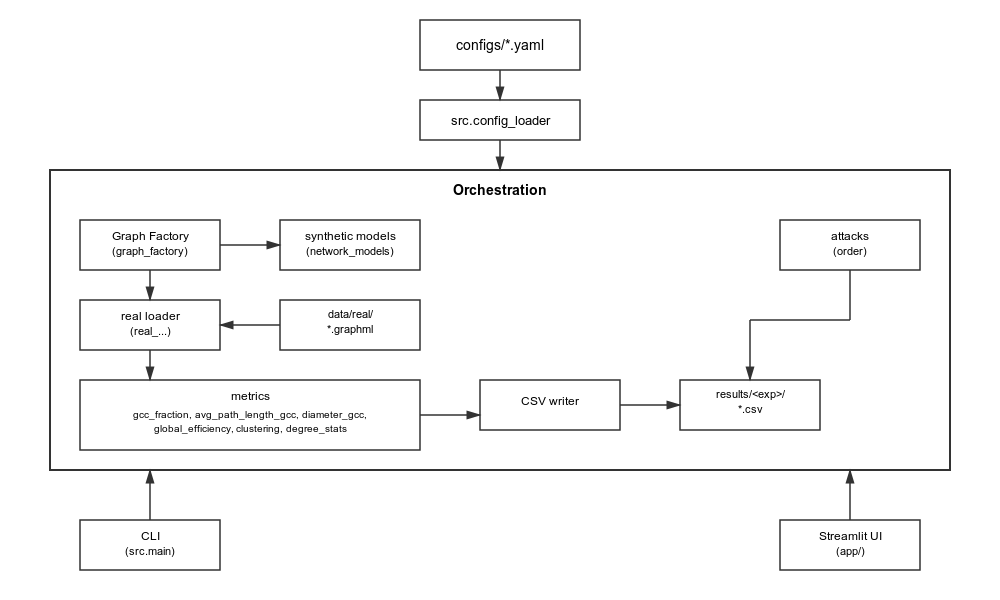
\includegraphics[width=\textwidth]{figures/architecture.png}
  \caption{Architektur des Simulationsprojekts. Die Simulation wird vollständig über
  Konfigurationsdateien gesteuert und modular in Netzwerkgenerierung,
  Angriffsszenarien, Metrikberechnung und Ergebnisverarbeitung unterteilt.}
  \label{fig:projektarchitektur}
\end{figure}


\paragraph{Konfigurations- und Steuerungsebene}
Die Konfiguration der Experimente erfolgt vollständig über YAML-Dateien. Das
Laden und Validieren dieser Konfigurationen wird durch das Modul
\texttt{src/config\_loader.py} realisiert. Dieses Modul stellt sicher, dass
alle benötigten Parameter vorhanden sind und in einer einheitlichen internen
Struktur an die weiteren Komponenten des Systems übergeben werden.\\
Die zentrale Steuerung eines Experiments erfolgt über das Modul
\texttt{src/simulation.py}. Dieses Modul koordiniert den gesamten Ablauf eines
Simulationslaufs, beginnend bei der Netzwerkgenerierung über die Anwendung der
Störungsszenarien bis hin zur Berechnung der Metriken und dem Speichern der
Ergebnisse. Dadurch fungiert \texttt{simulation.py} als verbindende Schicht
zwischen den einzelnen Funktionsmodulen.

\paragraph{Netzwerkgenerierung und Datenanbindung}
Die Erzeugung synthetischer Netzwerke ist im Modul \texttt{src/network\_models.py}
implementiert. Dort sind die verschiedenen Netzwerkmodelle (Erdős--Rényi,
Watts--Strogatz, Barabási--Albert) gekapselt, sodass sie über eine einheitliche
Schnittstelle instanziiert werden können. Für reale Netzwerke wird ein separater Ladepfad verwendet. \\
Das Modul \texttt{src/real\_network\_loader.py} übernimmt das Einlesen von GraphML-Dateien
sowie optionale Vorverarbeitungsschritte, etwa die Beschränkung auf die größte
verbundene Komponente oder die Umnummerierung der Knoten. Die Auswahl, ob ein
synthetisches oder reales Netzwerk erzeugt wird, erfolgt zentral über das Modul
\texttt{src/graph\_factory.py}, das als Abstraktionsschicht zwischen
Konfiguration und konkreter Netzwerkgenerierung dient.

\paragraph{Störungsszenarien und Angriffsauswahl}
Die Definition der Störungsszenarien ist im Modul \texttt{src/attacks.py}
umgesetzt. Dieses Modul berechnet für ein gegebenes Netzwerk die Reihenfolge,
in der Knoten im Rahmen eines bestimmten Angriffsszenarios entfernt werden
sollen. Dabei werden sowohl zufällige Ausfälle als auch gezielte Angriffe auf
Basis von Zentralitätsmaßen unterstützt.\\
Durch die Auslagerung der Angriffsauswahl in ein eigenes Modul wird eine klare
Trennung zwischen der Definition der Störung und ihrer Anwendung erreicht. Neue
Angriffsszenarien können so implementiert werden, ohne den Ablauf der
Simulation selbst verändern zu müssen.

\paragraph{Metrikberechnung und Analyse}
Die Berechnung aller strukturellen Metriken erfolgt im Modul
\texttt{src/metrics.py}. Dieses Modul enthält Funktionen zur Bestimmung der
Größe der größten verbundenen Komponente, von Clustering-Koeffizienten,
Durchmesser, Effizienz und weiteren Kenngrößen. Die Metrikfunktionen sind
bewusst unabhängig von der Simulation implementiert, sodass sie auch isoliert
auf einzelne Netzwerke angewendet werden können.\\
Die weiterführende Auswertung der Simulationsergebnisse, insbesondere die
Aggregation über mehrere Wiederholungen sowie die Berechnung der
Robustheitskennzahlen wie der Fläche unter der Robustheitskurve, erfolgt im
Modul \texttt{src/analysis.py}. Diese Trennung erleichtert eine saubere
Nachvollziehbarkeit der einzelnen Verarbeitungsschritte.

\paragraph{Visualisierung und Benutzeroberfläche}
Die grafische Benutzeroberfläche ist im Verzeichnis \texttt{app/} umgesetzt und
basiert auf Streamlit. Die Datei \texttt{streamlit\_app.py} verbindet die
Konfigurations-, Simulations- und Analysekomponenten zu einer interaktiven
Oberfläche. Neben tabellarischen und grafischen Auswertungen wird dort auch
eine dynamische Visualisierung der Netzwerkstruktur realisiert, die den
schrittweisen Zerfall des Netzwerks während der Simulation sichtbar macht.\\
Die eigentliche Logik zur dynamischen Netzvisualisierung ist im Modul \\
\texttt{src/dynamic\_visualization.py} gekapselt. Dadurch bleibt die
Benutzeroberfläche übersichtlich, während die Visualisierungslogik unabhängig
weiterentwickelt werden kann.

\paragraph{Architektonische Einordnung}
Die gewählte Architektur folgt keinem monolithischen Ansatz, sondern
orientiert sich an der logischen Trennung der experimentellen Aufgaben. Diese
Struktur unterstützt sowohl die Erweiterbarkeit des Projekts als auch dessen
Verständlichkeit. Gleichzeitig bleibt die Implementierung bewusst einfach
gehalten, um den Fokus auf die inhaltliche Analyse der Netzwerke und nicht auf
komplexe Softwarearchitektur zu legen.

\subsection{Reproduzierbarkeit und Konfigurationsmanagement}

Ein zentrales Ziel der Implementierung ist die vollständige
Reproduzierbarkeit aller durchgeführten Experimente. Da die Analyse komplexer
Netzwerke sowohl stochastische Prozesse als auch zufallsbasierte
Netzgenerierung umfasst, ist ein transparentes und konsistentes
Konfigurationsmanagement notwendig. Dieses wird im Projekt durch eine klare
Trennung von Code, Konfiguration und Ergebnisdaten realisiert.

\paragraph{Konfigurationsdateien}
Alle experimentellen Parameter werden ausschließlich über YAML-basierte
Konfigurationsdateien im Verzeichnis \texttt{configs/} definiert. Diese
Dateien enthalten sämtliche Informationen zur Beschreibung eines Experiments,
darunter die Auswahl der Netzwerkmodelle, deren Parametrisierung, die
betrachteten Störungsszenarien, die Schrittweite der Knotenentfernung sowie
die zu berechnenden Metriken.\\
Durch diese Auslagerung der Konfiguration aus dem Programmcode können neue
Experimente definiert oder bestehende Experimente variiert werden, ohne
Änderungen an der Implementierung vornehmen zu müssen. Gleichzeitig bleibt die
vollständige Beschreibung eines Experiments in einer einzelnen Datei
nachvollziehbar dokumentiert.

\paragraph{Zufallsstartwerte und deterministisches Verhalten}
Zur Kontrolle stochastischer Einflüsse werden alle zufallsbasierten Prozesse
durch explizite Zufallsstartwerte (Seeds) gesteuert. Diese betreffen sowohl
die Generierung synthetischer Netzwerke als auch die Auswahl zufälliger
Ausfallreihenfolgen bei Random-Failure-Szenarien. Die verwendeten Seeds sind
Bestandteil der jeweiligen Konfigurationsdateien.

Durch dieses Vorgehen ist sichergestellt, dass identische
Konfigurationsdateien bei mehrfacher Ausführung zu denselben Netzwerken,
Ausfallreihenfolgen und Simulationsergebnissen führen. Dies ermöglicht nicht
nur eine zuverlässige Reproduktion der Ergebnisse, sondern auch einen gezielten
Vergleich einzelner Parameteränderungen.

\paragraph{Ergebnisstruktur und Versionierung}
Die Ergebnisse der Simulationen werden automatisiert im Verzeichnis
\texttt{results/} abgelegt. Für jedes Experiment wird ein eigener Unterordner
erzeugt, der sowohl die Rohdaten der einzelnen Simulationsläufe als auch
aggregierte Auswertungen enthält. Die Dateinamen enthalten den Namen des
Experiments, sodass eine eindeutige Zuordnung zwischen Konfiguration und
Ergebnisdaten möglich ist.\\
Die Speicherung der Ergebnisse in tabellarischer Form ermöglicht eine spätere
Weiterverarbeitung, etwa für zusätzliche Analysen oder externe
Visualisierungen. In Kombination mit einer Versionsverwaltung des Quellcodes
lassen sich so auch ältere Ergebnisse eindeutig einem bestimmten Stand der
Implementierung zuordnen.

\paragraph{Nachvollziehbarkeit des Experimentablaufs}
Durch die Kombination aus konfigurationsbasierter Steuerung, deterministischer
Simulation und strukturierter Ergebnisablage ist der gesamte Experimentablauf
transparent nachvollziehbar. Jeder Schritt von der Definition der Parameter
bis zur Auswertung der Ergebnisse lässt sich rekonstruieren. Dieses Vorgehen
entspricht gängigen wissenschaftlichen Standards und stellt sicher, dass die
im Rahmen dieser Arbeit präsentierten Ergebnisse überprüfbar und
reproduzierbar sind.



\section{Ergebnisse}

\subsection{Topologische Eigenschaften der untersuchten Netzwerke}

Bevor die Robustheit der Netzwerke unter Störungen analysiert wird, ist es
sinnvoll, die grundlegenden topologischen Eigenschaften der betrachteten
Netzwerke zu vergleichen. Diese Eigenschaften bestimmen maßgeblich, wie ein
Netzwerk auf Knotenentfernungen reagiert. Die Analyse bezieht sich auf den
Ausgangszustand der Netzwerke ohne Knotenentfernung ($q = 0$), der in den
Simulationsdaten explizit enthalten ist.\\
Untersucht werden drei synthetische Netzwerkmodelle: ein Erdős--Rényi-Zufallsgraph
(ER), ein Watts--Strogatz-Small-World-Netzwerk (WS) und ein
Barabási--Albert-Netzwerk (BA). Alle Netzwerke besitzen dieselbe Knotenzahl
($n=800$), wodurch strukturelle Unterschiede direkt vergleichbar sind.

\paragraph{Gradstruktur und Vernetzung}
Die drei Modelle unterscheiden sich deutlich in ihrer Gradstruktur. Der
Erdős--Rényi-Graph weist eine relativ homogene Gradverteilung auf: die meisten
Knoten besitzen einen ähnlichen Grad, extreme Abweichungen sind selten. Das
Watts--Strogatz-Netzwerk ist ebenfalls vergleichsweise homogen, besitzt aber
durch seine Ausgangsringstruktur eine deutlich stärkere lokale Vernetzung. Beim
Barabási--Albert-Netzwerk ist die Gradverteilung stark heterogen: wenige Knoten
fungieren als Hubs mit sehr hohem Grad, während der Großteil nur schwach
vernetzt ist. Diese Hub-Struktur ist für skalenfreie Netze typisch und wirkt
sich später stark auf die Robustheit unter gezielten Angriffen aus.

\paragraph{Clustering und lokale Struktur}
Ein zentraler Unterschied zeigt sich im Clustering. Das Watts--Strogatz-Netzwerk
besitzt sowohl einen hohen globalen Clustering-Wert als auch hohe mittlere
lokale Clustering-Koeffizienten. Das bestätigt die typische Small-World-Logik:
lokal dicht, global trotzdem kurze Wege. Der Erdős--Rényi-Graph hat dagegen nur
geringe Clustering-Werte; lokale Dreiecke entstehen hier eher zufällig. Das
Barabási--Albert-Netzwerk liegt dazwischen: es kann lokal durchaus Clustering
zeigen, jedoch ungleich verteilt (oft stärker um zentrale Knoten herum).

\paragraph{Pfadlängen und Durchmesser}
Mittlere kürzeste Pfadlänge und Durchmesser geben einen Eindruck der globalen
Erreichbarkeit. Erdős--Rényi und Watts--Strogatz zeigen im Ausgangszustand kurze
mittlere Pfadlängen. Beim Watts--Strogatz-Modell ist interessant, dass diese
kurzen Wege trotz hoher lokaler Struktur entstehen. Das Barabási--Albert-Netz
weist ebenfalls kurze Pfadlängen auf, was vor allem an den Hubs liegt, über die
viele kürzeste Wege laufen. Der Durchmesser ist dabei ein empfindlicherer
Indikator: er bleibt oft moderat, kann aber bei strukturellen Eingriffen schnell
ansteigen, wenn zentrale Vermittlerknoten verloren gehen.

\paragraph{Einordnung für die Robustheitsanalyse}
Diese topologischen Unterschiede bilden die Ausgangslage für die folgenden
Robustheitsanalysen. Homogene Gradverteilungen (ER, teilweise WS) sprechen für
eine gleichmäßigere Reaktion auf zufällige Ausfälle. Hohe lokale Clusterbildung
(WS) deutet auf Redundanz im Nahbereich hin. Die Hub-Struktur (BA) lässt
hingegen eine starke Robustheit bei Random Failures, aber eine hohe
Verwundbarkeit bei gezielten Angriffen erwarten. Ob und wie deutlich sich das
in den Simulationen zeigt, wird in den nächsten Unterabschnitten mit
Robustheitskurven und AUC-Kennzahlen überprüft.

\subsection{Robustheit unter zufälligen Ausfällen}

In diesem Abschnitt wird das Robustheitsverhalten der untersuchten
Netzwerkmodelle unter zufälligen Knotenausfällen analysiert. Zufällige Ausfälle
modellieren Störungen ohne gezielte Auswahl einzelner Knoten, wie sie etwa durch
technische Defekte oder lokale externe Einwirkungen auftreten können. Zur
Bewertung wird die Konnektivität der verbleibenden Netzwerke in Abhängigkeit vom
Anteil entfernter Knoten betrachtet.\\
Als zentrale Metrik wird die Größe der größten verbundenen Komponente relativ zur
Anzahl der verbleibenden Knoten verwendet,
\[
S_{\text{surv}}(q) = \frac{|\mathrm{GCC}(q)|}{N - n_{\text{removed}}(q)}.
\]
Diese Normalisierung erlaubt es, Fragmentierungseffekte von dem trivialen Effekt
der Knotenentfernung zu trennen und die strukturelle Kohärenz unter den
verbleibenden Knoten gezielt zu untersuchen.\\
Abbildung~\ref{fig:random_failures_survivors} zeigt die resultierenden
Robustheitskurven für Erdős--Rényi-, Watts--Strogatz- und
Barabási--Albert-Netzwerke. Für kleine und mittlere Ausfallgrade bleibt die
Konnektivität in allen drei Modellen nahezu vollständig erhalten. Erst bei hohen
Werten von $q$ kommt es zu einer deutlichen Fragmentierung der Netzwerke.\\
Zwischen den Modellen lassen sich dennoch systematische Unterschiede erkennen.
Das Erdős--Rényi-Netzwerk weist über einen großen Bereich von $q$ die höchste
Konnektivität unter den verbleibenden Knoten auf. Die Fragmentierung setzt hier
erst relativ spät ein. Das Watts--Strogatz-Netzwerk zeigt demgegenüber einen
früheren und steileren Abfall von $S_{\text{surv}}(q)$. Trotz hoher lokaler
Clusterbildung führen zufällige Ausfälle bei größeren Ausfallgraden schneller
zu einer Aufspaltung des Netzwerks. Das Barabási--Albert-Netzwerk nimmt eine
Zwischenposition ein: Die Konnektivität bleibt zunächst stabil, sinkt jedoch bei
hohen Ausfallgraden stärker als im Erdős--Rényi-Fall.\\
Insgesamt zeigt sich, dass unter zufälligen Ausfällen alle betrachteten
Netzwerkmodelle eine vergleichsweise hohe Robustheit aufweisen. Die beobachteten
Unterschiede sind moderat und treten überwiegend erst bei großen Ausfallgraden
auf. Dieses Ergebnis steht im Einklang mit theoretischen Erwartungen und
unterstreicht, dass zufällige Störungen allein nur begrenzt geeignet sind, um
strukturelle Verwundbarkeiten deutlich sichtbar zu machen. Eine wesentlich
stärkere Differenzierung ist bei gezielten Angriffen zu erwarten, die im
folgenden Abschnitt untersucht werden.

\begin{figure}[htbp]
  \centering
  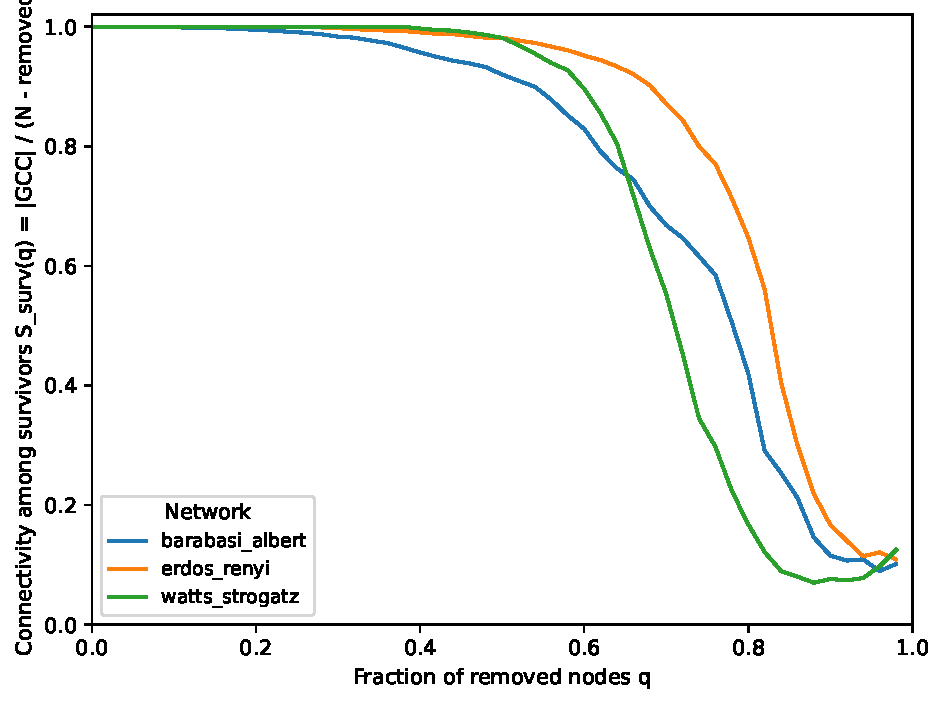
\includegraphics[width=0.9\textwidth]{figures/abb5_random_failures_survivors.pdf}
  \caption{Konnektivität der verbleibenden Knoten unter zufälligen
  Knotenausfällen. Dargestellt ist die normierte Größe der größten verbundenen
  Komponente relativ zur Anzahl der verbleibenden Knoten
  $S_{\text{surv}}(q)=|\mathrm{GCC}(q)|/(N-n_{\text{removed}})$.}
  \label{fig:random_failures_survivors}
\end{figure}


\subsection{Robustheit unter gezielten Angriffen}

In diesem Abschnitt wird das Robustheitsverhalten der untersuchten Netzwerke
unter gezielten Angriffen analysiert. Im Gegensatz zu zufälligen Ausfällen
werden hierbei Knoten nicht zufällig, sondern anhand struktureller
Zentralitätsmaße entfernt. Solche Szenarien modellieren bewusste Angriffe auf
kritische Netzkomponenten und stellen eine Worst-Case-Betrachtung der
Netzwerkstabilität dar.\\
Untersucht werden zwei Angriffstypen: gezielte Angriffe auf Basis des
Knotengrads sowie auf Basis der Betweenness-Zentralität. In beiden Fällen werden
Knoten iterativ in absteigender Reihenfolge des jeweiligen Zentralitätsmaßes
entfernt.

\paragraph{Gradbasierte Angriffe}
Abbildung~\ref{fig:targeted_degree} zeigt die Robustheitskurven unter
gradbasierten Angriffen. Die Unterschiede zwischen den Netzwerkmodellen sind in
diesem Szenario besonders deutlich ausgeprägt. Das Barabási--Albert-Netzwerk
reagiert extrem empfindlich auf die gezielte Entfernung hochgradiger Knoten.
Bereits bei kleinen Anteilen entfernter Knoten bricht die größte verbundene
Komponente nahezu vollständig zusammen.\\
Ursächlich hierfür ist die ausgeprägte Hub-Struktur skalenfreier Netzwerke. Die
Entfernung weniger zentraler Knoten führt dazu, dass große Teile des Netzwerks
ihre Anbindung verlieren. Erdős--Rényi- und Watts--Strogatz-Netzwerke zeigen
demgegenüber eine deutlich höhere Robustheit. Aufgrund ihrer homogeneren
Gradverteilungen erfolgt die Fragmentierung hier schrittweise und erst bei
höheren Angriffsstärken.

\begin{figure}[htbp]
  \centering
  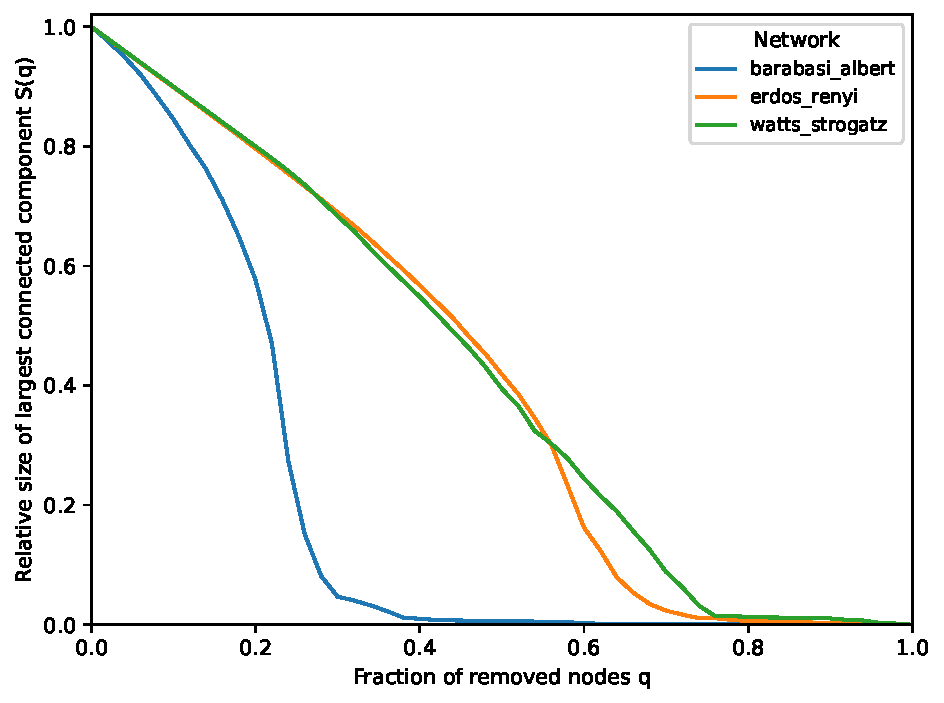
\includegraphics[width=0.9\textwidth]{figures/abb5_targeted_degree_curves.pdf}
  \caption{Robustheitskurven der untersuchten Netzwerkmodelle unter gezielten
  Angriffen auf Basis des Knotengrads.}
  \label{fig:targeted_degree}
\end{figure}

\paragraph{Angriffe nach Betweenness-Zentralität}
Die Auswirkungen gezielter Angriffe auf Basis der Betweenness-Zentralität sind
in Abbildung~\ref{fig:targeted_betweenness} dargestellt. Auch in diesem Szenario
zeigt das Barabási--Albert-Netzwerk eine ausgeprägte Verwundbarkeit. Die
Entfernung weniger Knoten mit hoher Vermittlungsfunktion führt rasch zu einer
Fragmentierung des Netzwerks.\\
Auffällig ist zudem das Verhalten des Watts--Strogatz-Netzwerks. Trotz hoher
lokaler Clusterbildung reagieren diese Netzwerke empfindlich auf
Betweenness-basierte Angriffe, da einzelne Knoten eine zentrale Rolle für die
Verbindung verschiedener Netzwerkbereiche einnehmen. Erdős--Rényi-Netzwerke
weisen auch in diesem Szenario die höchste Robustheit auf, da keine einzelnen
Knoten eine dominierende Vermittlungsfunktion besitzen.

\begin{figure}[htbp]
  \centering
  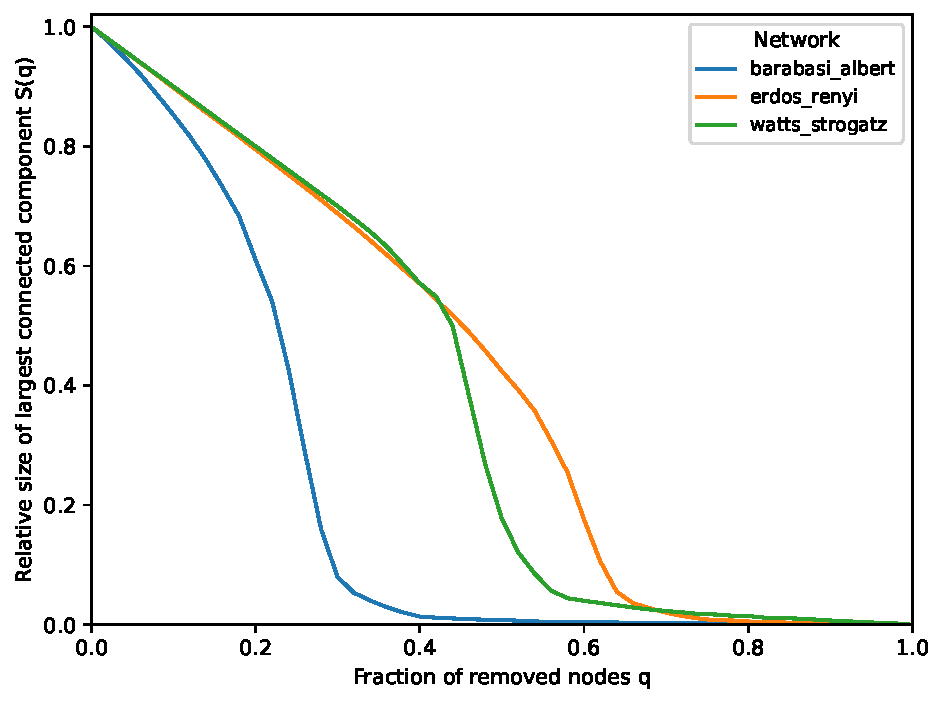
\includegraphics[width=0.9\textwidth]{figures/abb5_targeted_betweenness_curves.pdf}
  \caption{Robustheitskurven der untersuchten Netzwerkmodelle unter gezielten
  Angriffen auf Basis der Betweenness-Zentralität.}
  \label{fig:targeted_betweenness}
\end{figure}

\paragraph{Zusammenfassende Einordnung}
Der Vergleich beider Angriffsszenarien zeigt, dass gezielte Angriffe die
Netzwerkstruktur wesentlich stärker beeinträchtigen als zufällige Ausfälle.
Insbesondere skalenfreie Netzwerke, die unter Random Failures als robust gelten,
erweisen sich unter gezielten Angriffen als hochgradig verwundbar. Die
Simulationen bestätigen damit zentrale theoretische Befunde und verdeutlichen,
dass strukturelle Zentralität ein entscheidender Faktor für die Stabilität
komplexer Netzwerke ist.

\subsection{Zusammenfassender Robustheitsvergleich mittels AUC}

Die bisherigen Abschnitte haben das Robustheitsverhalten der Netzwerke anhand
von Kurvenverläufen illustriert. Für einen kompakten und vergleichbaren
Gesamtüberblick wird im Folgenden die Fläche unter der Robustheitskurve (Area
Under the Curve, AUC) betrachtet. Als zugrunde liegende Größe dient dabei
\[
S(q) = \frac{|\mathrm{GCC}(q)|}{N},
\]
also der relative Anteil der größten verbundenen Komponente in Abhängigkeit vom
entfernten Knotenantteil $q$. Die AUC fasst den gesamten Kurvenverlauf zu einer
einzigen Kennzahl zusammen und erlaubt damit einen direkten quantitativen
Vergleich zwischen Netzwerken und Angriffsszenarien.

\begin{table}[htbp]
\centering
\caption{AUC der Robustheitskurven (größere Werte $\Rightarrow$ höhere Robustheit).}
\label{tab:auc_summary}
\begin{tabular}{lccc}
\hline
Netzwerk & Random Failures & Targeted (Degree) & Targeted (Betweenness) \\
\hline
BA\_n800\_m3 & 0.454 & 0.196 & 0.210 \\
ER\_n800\_p0.01 & 0.476 & 0.408 & 0.407 \\
WS\_n800\_k8\_p0.1 & 0.454 & 0.418 & 0.375 \\
\hline
\end{tabular}
\end{table}


\paragraph{Random Failures}
Unter zufälligen Ausfällen zeigen alle drei synthetischen Netzwerkmodelle
vergleichsweise hohe AUC-Werte. Das Erdős--Rényi-Netzwerk weist mit
$\mathrm{AUC}\approx0{,}48$ die höchste Robustheit auf, gefolgt von
Watts--Strogatz und Barabási--Albert mit nahezu identischen Werten von rund
$0{,}45$. Dieses Ergebnis spiegelt die relativ homogene Struktur der ER-Netze
wider, bei denen zufällige Knotenausfälle die globale Konnektivität erst spät
beeinträchtigen. Gleichzeitig zeigt sich, dass auch skalenfreie Netze bei
ungerichteten Störungen keine besondere strukturelle Schwäche aufweisen.

\paragraph{Gezielte Angriffe nach Knotengrad}
Bei gradbasierten Angriffen tritt ein deutlich anderes Bild auf. Das
Barabási--Albert-Netzwerk bricht frühzeitig zusammen und erreicht mit einer AUC
von etwa $0{,}20$ den mit Abstand niedrigsten Wert. Erdős--Rényi- und
Watts--Strogatz-Netzwerke bleiben dagegen deutlich stabiler
($\mathrm{AUC}\approx0{,}41$). Dieses Ergebnis bestätigt quantitativ die in der
Literatur bekannte hohe Verwundbarkeit skalenfreier Netzwerke gegenüber
gezielten Angriffen auf hochgradige Knoten.

\paragraph{Gezielte Angriffe nach Betweenness}
Auch bei Angriffen auf Knoten mit hoher Betweenness-Zentralität zeigt sich eine
starke Differenz zwischen den Modellen. Das Barabási--Albert-Netzwerk erreicht
erneut nur eine sehr geringe AUC von etwa $0{,}21$, während Erdős--Rényi mit
$\mathrm{AUC}\approx0{,}41$ und Watts--Strogatz mit etwa $0{,}38$ deutlich robuster
bleiben. Im Vergleich zum gradbasierten Angriff fällt der Unterschied zwischen
ER und WS hier stärker ins Gewicht, was auf die Bedeutung vermittelnder
Knotenpositionen in Small-World-Strukturen hindeutet.

\paragraph{Gesamtbewertung}
Die AUC-Auswertung bestätigt die zuvor beobachteten Kurvenverläufe in
kompakter Form. Skalenfreie Netzwerke sind gegenüber zufälligen Ausfällen
vergleichsweise robust, reagieren jedoch extrem empfindlich auf gezielte
Angriffe. Erdős--Rényi- und Watts--Strogatz-Netze zeigen dagegen ein insgesamt
ausgeglicheneres Robustheitsverhalten über alle Szenarien hinweg. Die geringe
Streuung der AUC-Werte über die Wiederholungen hinweg unterstreicht zudem die
Stabilität der beobachteten Effekte.

\bibliographystyle{plainnat}
\bibliography{literatur}

\end{document}
